\documentclass[dvipdfmx,autodetect-engine,titlepage]{jsarticle}
\usepackage[dvipdfm]{graphicx}
\usepackage{ascmac}
\usepackage{fancybox}
\usepackage{listings}
\usepackage{plistings}
\usepackage{itembkbx}
\usepackage{amsmath}
\usepackage{svg}
\usepackage{url}
\usepackage{graphics}
\usepackage{listings,jvlisting}

\textheight=23cm
\renewcommand{\figurename}{図}
\renewcommand{\tablename}{表}
\newenvironment{code}
{\vspace{0.5zw}\VerbatimEnvironment  
\begin{screen} 
\baselineskip=1.0\normalbaselineskip
 \begin{Verbatim}}
{\end{Verbatim}
\baselineskip=\normalbaselineskip
 \end{screen}\vspace{0.5zw}} 

\title{情報理工学部 SNコース 3回\\
自然言語処理第10回講義レポート\\}
\author{2600200443-6\\Yamashita Kyohei\\山下 恭平}
\date{Jun 17 2022}

\begin{document}

\maketitle

\section{とく}

\begin{figure}[h]
  \centering
  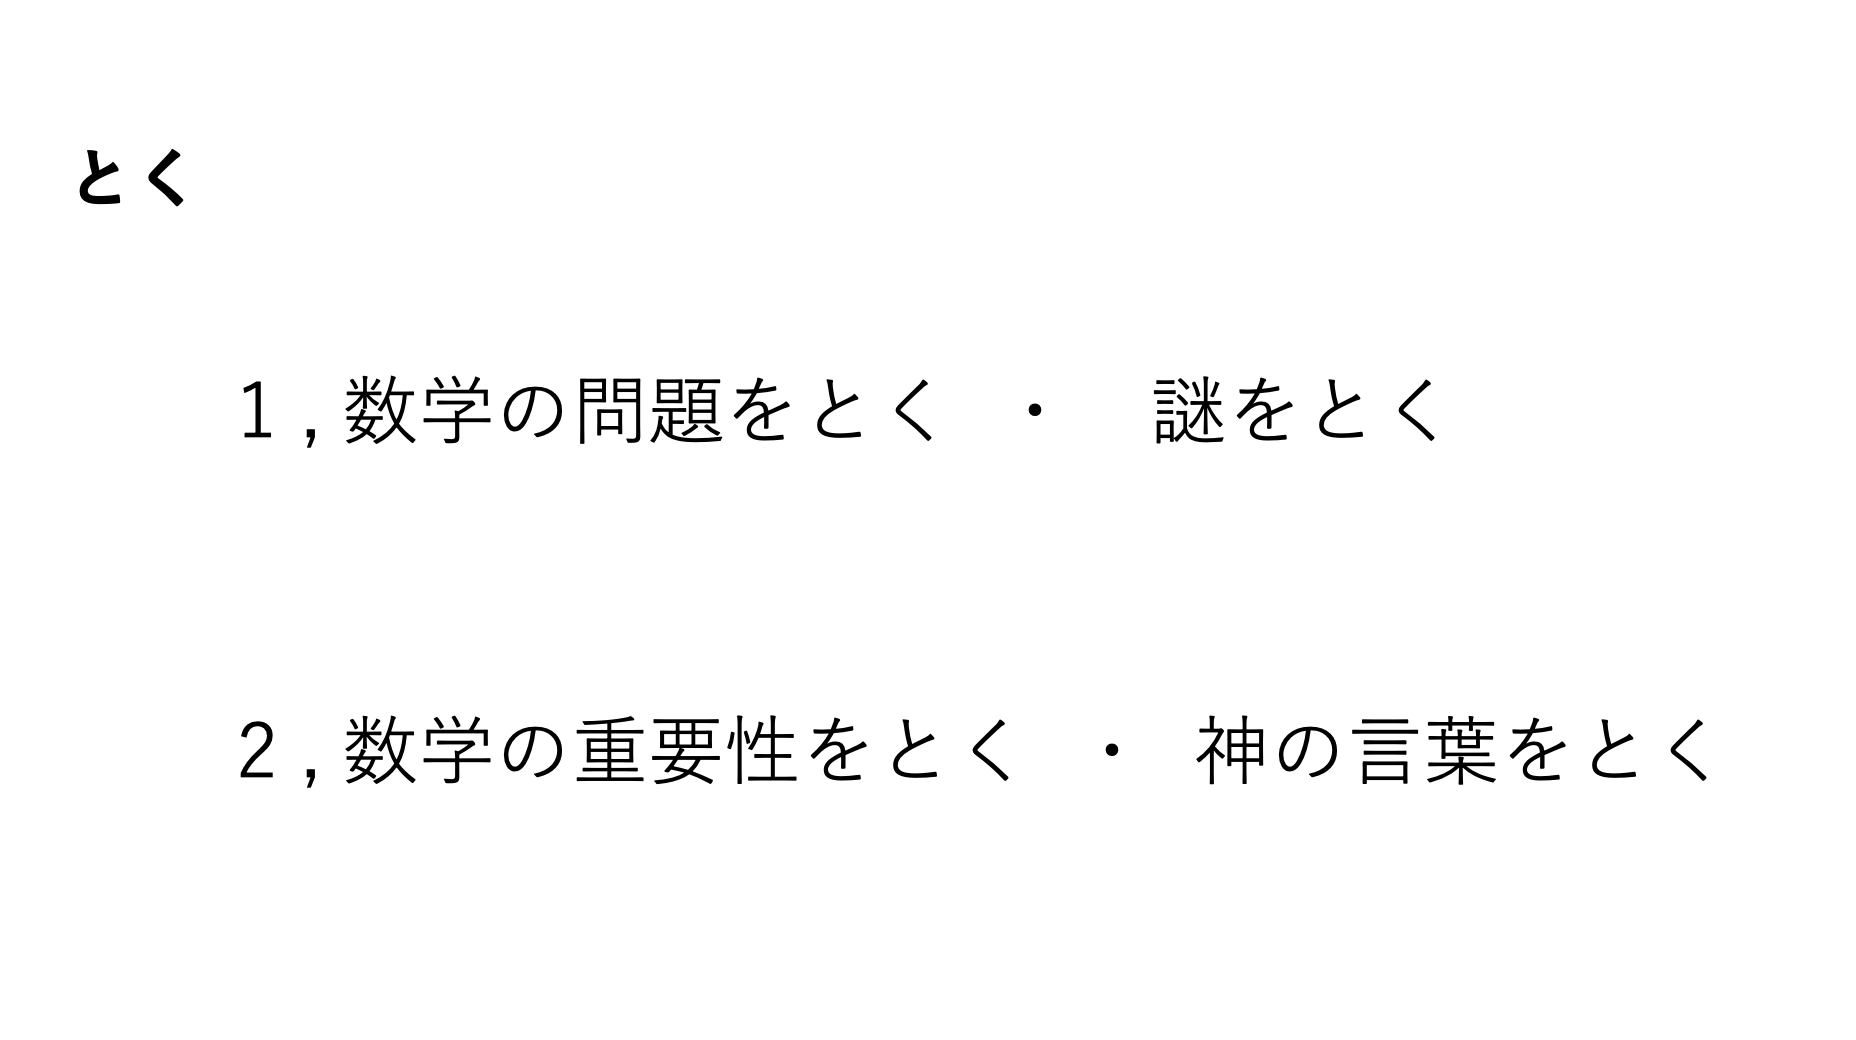
\includegraphics[scale=0.5]{pic1.png}
\end{figure}

\subsection*{解説}

1の「とく」は対象がとかれる事により、未知の事柄に対する「答え」が得られる。
そのためとかれる対象は、未知のものであることが求められ、また、とかれた結果は一意
に定まることが多い。英語では「solve」で訳されることが多い。
\begin{quote}
  \begin{itemize}
   \item 運動靴の紐をとく。
   \item 連立方程式をとく。
   \item この問題はとくことができない。
  \end{itemize}
 \end{quote}

2の「とく」は自分以外の人物に、対象について「とく」ことで、相手への理解を促す。
説明すること。そのため対象は、漠然としたもの、抽象的なものであることが多い。
また、とかれた結果により起こる変化は人の心境の変化など、目に見えないことが
多い。英語では「explain」と訳されることが多い。
\begin{quote}
  \begin{itemize}
   \item 説法をとく。
   \item 世界平和についてとく。
   \item 駅で謎のおじさんに社会正義についてとかれた。
  \end{itemize}
 \end{quote}

\newpage

\section{みる}

\begin{figure}[h]
  \centering
  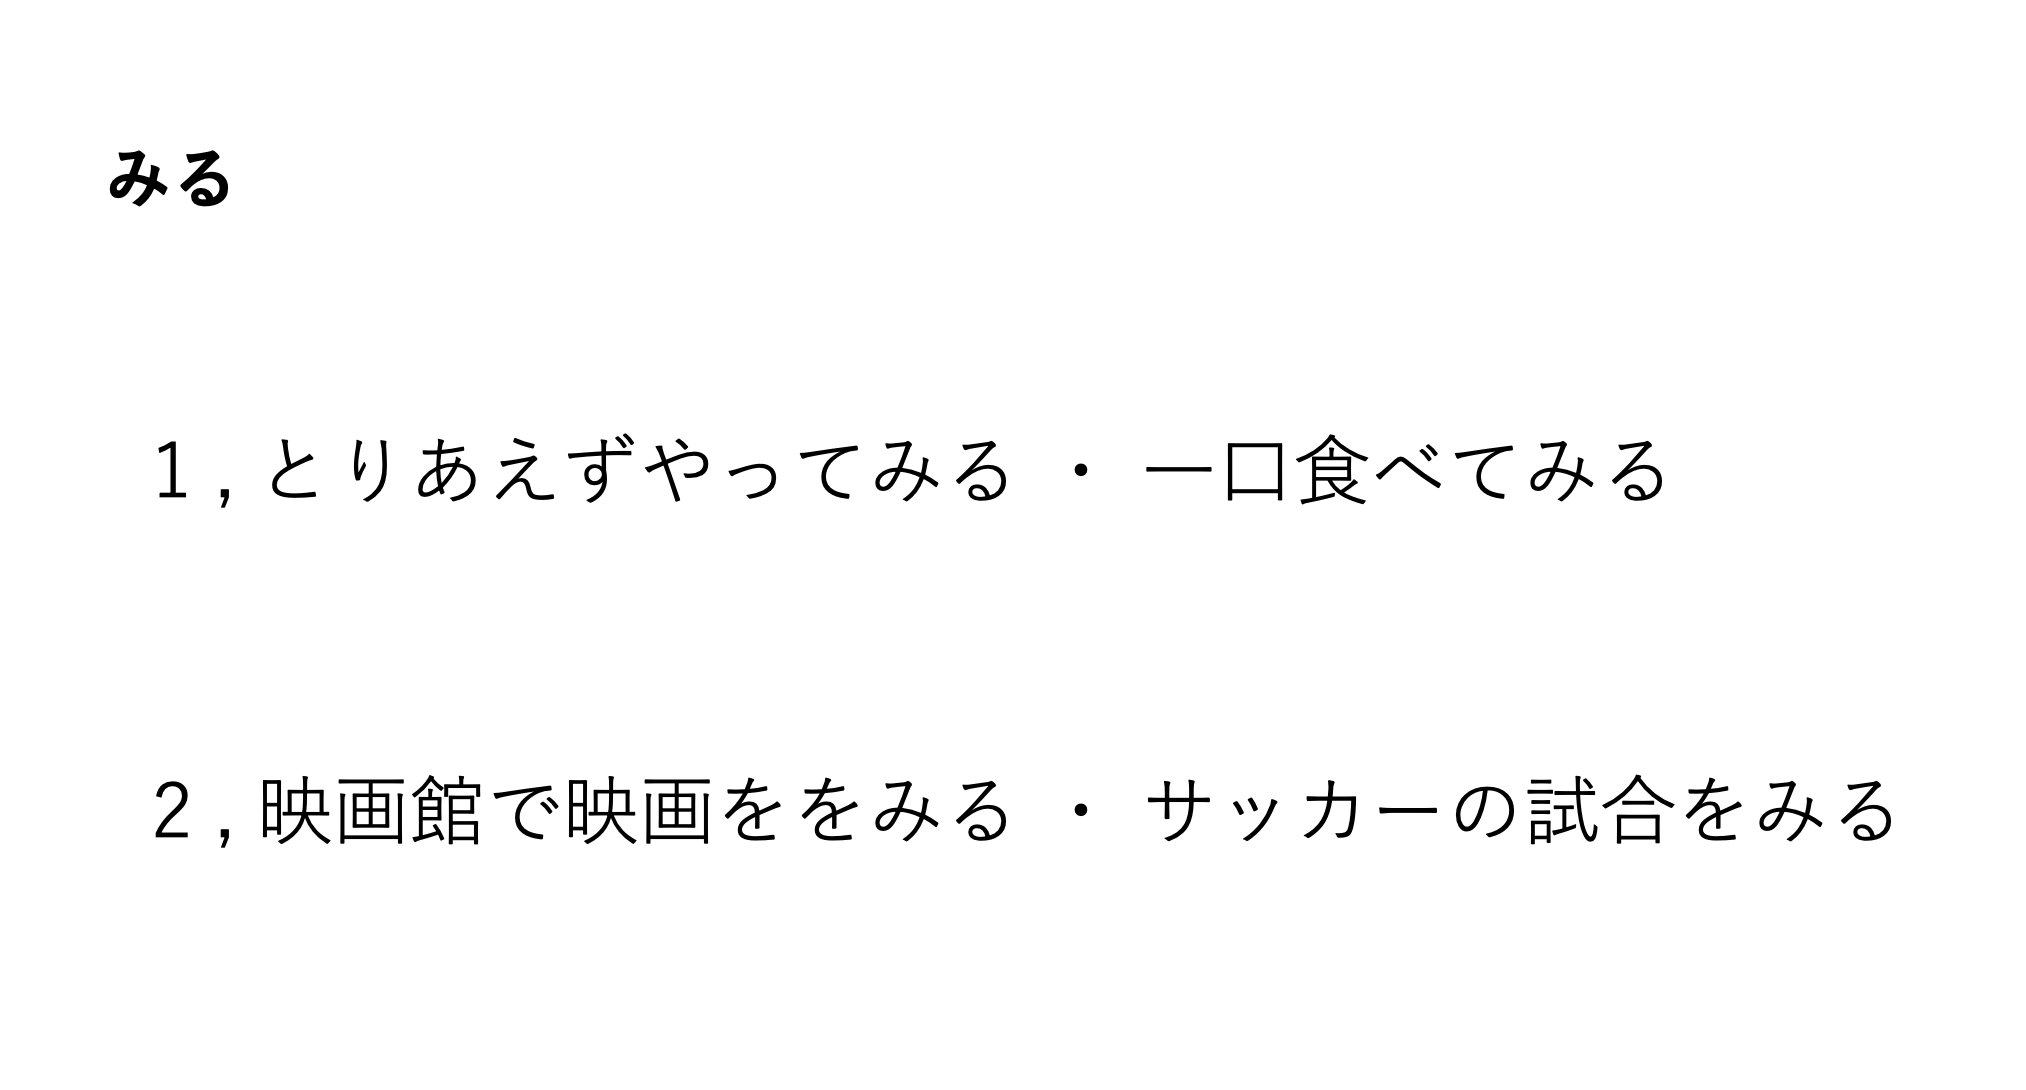
\includegraphics[scale=0.4]{pic2.png}
\end{figure}


\subsection*{解説}

1の「みる」は「試みる」であり、何らかの動作、行為を指す。また、行われる
動作は、非計画的なものや、テスト段階であることが多い。「みる」というが視覚
を用いた動作を指すわけではない。英語では「try」と訳される。
\begin{quote}
  \begin{itemize}
   \item ノープランで旅行に行ってみる。
   \item 新しい企画を発案してみる。
   \item サイズが合うかわからないので着てみる。
  \end{itemize}
 \end{quote}

2の「みる」は「見る」であり、対象を「見る」つまりは、視覚からの情報を得る
ことを指す。視覚からの情報を得る行為であるので、「みる」対象はかなり多岐に
渡る。今回の例文ではどちらも「観察する、閲覧する」の見るにあたり英語では「watch」
と訳される。
\begin{quote}
  \begin{itemize}
   \item ネットフリックスをみる。
   \item 熱い戦いをみる。
   \item 草原で走る犬をみる。
  \end{itemize}
 \end{quote}

\end{document}